\documentclass[9pt]{article}
\usepackage[utf8]{inputenc}
\usepackage{amsmath,amsthm,amsfonts,amssymb,amscd}
\usepackage{multirow,booktabs}
\usepackage{enumitem}
\usepackage{fancyhdr}
\usepackage{mathrsfs}
\usepackage{wrapfig}
\usepackage{setspace}
\usepackage{calc}
\usepackage{multicol}
\usepackage{cancel}
\usepackage[retainorgcmds]{IEEEtrantools}
\usepackage{framed}
\usepackage[most]{tcolorbox}
\usepackage{tikz}
\usepackage{geometry}
\geometry{
	a4paper,
	total={170mm,257mm},
	left=20mm,
	top=20mm,
}
\title{Planetary Motion}
\author{Aaron G.K.}

\begin{document}
	\maketitle
	\begin{center}
		\section*{Kepler's Laws of Planetary Motion}	
	\end{center}
	
	In the past people used to think the Earth was the center of the universe(Geocentric worldview) with all the other celestial bodies revolving around us. If you ever had a chance to look at the night sky a couple of nights consecutively you'd recognize the paths of some of the stars and it is indeed circular and they seem to be rotating around us, however, it was only after the days of Galilee and Newton that we were able to recognize that we revolve around the sun in the solar system(Heliocentric view) and not the other way around. With Newton's idea of universal gravitation, a lot of new ideas emerged about the motion of planets. A Danish astronomer, Tycho Brahe, collected information about planets  plotting their positions at regular intervals of time. Johannes Kepler, made careful analysis from the data Brahe left and he formulated three important laws about planetary motion. \\
	
	\subsection*{Kepler's First Law}
	Newton proved that as gravity decreases with distance by a factor of $\frac{1}{r^2}$, closed orbits must have the form of an ellipse or circle while open orbits could be hyperbolic or parabolic. All motion caused by an inverse square force is one of the four conic sections and is determined by the \textbf{energy} and \textbf{direction} of the moving body. The four conic sections are shown below:
	\begin{center}
		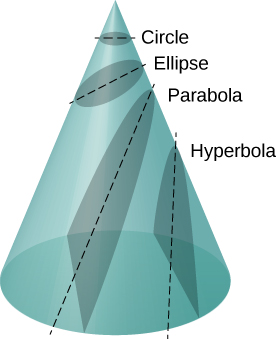
\includegraphics[scale=0.7]{conic_sections.jpeg}
	\end{center}
	The dominant view during Kepler's time was that planetary motion was circular. When Kepler tried fitting Tyco Brahe's data onto circular orbits, it just wouldn't work - Mars especially was the biggest challenge to this view. When he tried working with another conic sections instead of a circle, it worked for him. \textbf{Kepler's First Law} states that the paths of planets around the sun is elliptical with the sun being located at one focus. An ellipse is a conic section such that the sum of the distance from the foci stays constant. 
	\begin{center}
		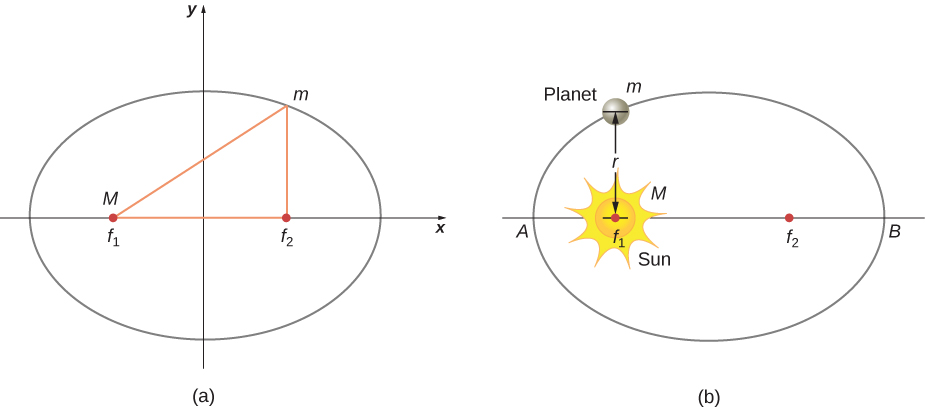
\includegraphics[scale=0.7]{ellipse.jpeg}
	\end{center}
	For elliptical orbits, the point of closest approach of a planet to the Sun is called the \textit{perihelion}. It is labeled point A in the figure above. The farthest point is the \textit{aphelion} and is labeled point B in the figure. For the Moon’s orbit about Earth, those points are called the \textit{perigee} and \textit{apogee}, respectively.
	\subsection*{Kepler's Second Law}
	 Kepler’s second law states that a planet sweeps out equal areas in equal times, that is, the area divided by time, called the areal velocity, is constant. Consider the figure below. The time it takes a planet to move from position A to B, sweeping out area $A1$, is exactly the time taken to move from position C to D, sweeping area $A2$, and to move from E to F, sweeping out area $A3$. These areas are the same: $A1=A2=A3$.
	\begin{center}
		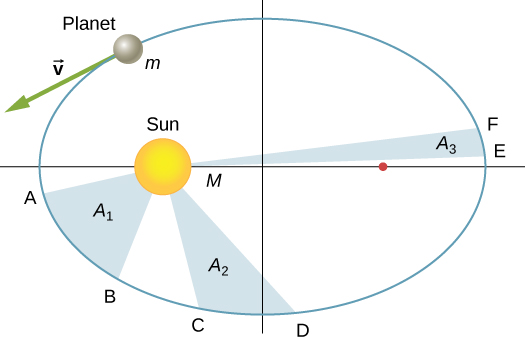
\includegraphics[scale=0.7]{areal_velocity.jpeg}
	\end{center}
	Comparing the areas in the figure and the distance traveled along the ellipse in each case, we can see that in order for the areas to be equal, the planet must speed up as it gets closer to the Sun and slow down as it moves away. It is the result of the Conservation of Angular Momentum - since the angular momentum is constant, the areal velocity must also be constant. As with Kepler’s first law, Newton showed it was a natural consequence of his law of gravitation.
	\subsection*{Kepler's Third Law}
	Kepler’s third law states that the square of the period is proportional to the cube of the semi-major axis of the orbit. We can also precisely state it in the following manner. \begin{quotation}
		The period, \textbf{T}, of a planet increases as its mean distance from the sun, \textbf{R}, raised to the $\frac{3}{2}$ power
	\end{quotation}
	The proof for this law is actually very simple - we have seen the steps needed for it during the discussion of Orbital Velocity while learning about Gravity. Again, we make the not-so-perfect assumption that planets travel in circular paths(just to make the proofs simpler), and we arrive at the fact that the force that keeps them in motion is the centripetal force. We do know, from Newton's Law of Universal Gravitation, that gravity is what causes the planets to orbit the Sun. Thus, we have the following be true:
	$$\dfrac{GmM}{r^2}=\dfrac{mv^2}{r}\text{,    where m is the mass of the planet and M is mass of the sun}$$
	We can express the velocity, $v$, in terms of the orbital period and the mean distance it has from the sun as follows:
	$$v=r\omega$$
	$$v=r\dfrac{\varDelta\theta}{\varDelta t}$$ For an orbit around the sun, the angular displacement is 1 revolution and we define the time it takes to make a revolution as the period, T. Thus, we have the following:
	$$v=r(\dfrac{1 \text{ rev}}{T})=r(\dfrac{2\pi\text{ rad}}{T})$$
	$$v=\dfrac{2\pi\text{r}}{\text{T}}$$
	Let's go back to our equation above and we can simplify it as follows:
    $$\dfrac{GM}{r}=v^2$$
    $$\dfrac{GM}{r}=(\dfrac{2\pi\text{r}}{\text{T}})^2$$
    $$\dfrac{GM}{r}=\dfrac{4\pi^2\text{r}^2}{\text{T}^2}$$
    $$GM\text{T}^2=4\pi^2\text{r}^3$$
    $$\text{T}^2=\dfrac{4\pi^2}{GM}r^3$$
\end{document}	